% !TEX TS-program = LaTeX-shellescape
\documentclass[a4paper]{article}

\usepackage[dutch]{babel}
\usepackage{geometry}
\usepackage{siunitx} % voor m/s, graden Celsius
\usepackage{parskip} % geen tab na paragraafeinde
\usepackage{amsmath, amssymb} % voor equation*
\usepackage[version=4]{mhchem} % chemie
\usepackage{graphicx} % afbeeldingen
\usepackage{fancyhdr} % headers en footers
\usepackage{xcolor} % kleuren
\usepackage{pdfpages} % pdf appenden
\usepackage[bookmarksnumbered]{hyperref} % links naar tabellen en figuren
\usepackage{minted}
\usepackage[normalem]{ulem} % strikethrough
\usepackage{mdframed}
\mdfsetup{skipabove=10pt,skipbelow=10pt}
\usepackage{booktabs}

\definecolor{indigo}{rgb}{0.0, 0.25, 0.42}

\hypersetup{
  colorlinks   = true, %Colours links instead of ugly boxes
  linkcolor    = blue, %Colour of internal links
  citecolor	   = blue
}

\newcommand{\red}{\textcolor{red}}
\newcommand{\orange}{\textcolor{orange}}
\newcommand{\yellow}{\textcolor{yellow}}
\newcommand{\green}{\textcolor{green}}
\newcommand{\blue}{\textcolor{blue}}
\newcommand{\indigo}{\textcolor{indigo}}
\newcommand{\violet}{\textcolor{violet}}

\newcommand{\Ums}{[\si[per-mode=symbol]{\meter\per\second}]}
\newcommand{\Um}{[\si{\meter}]}

\newminted[ltx]{latex}{fontsize=\footnotesize, frame=single, escapeinside=||}
\newmintinline[ltxi]{latex}{}


\begin{document}
\section{Starten met \LaTeX}
\subsection{Overleaf}
Maak een account aan op \href{https://www.overleaf.com}{Overleaf}. Klik op `Create First Project' $\rightarrow$ Blank Project. Geef het project de naam `LaTeX Workshop Aardwetenschappen'. Verwijder de code in het vak Source. 

\subsection{Een eenvoudig document}
Maak een document van de klasse \emph{article}. Gebruik a4-papier. Maak een aantal sections met \ltxi/\section/, \ltxi/\subsection/ en \ltxi/\paragraph/. Klik regelmatig op de knop \emph{Recompile} om te tussendoor te compileren.
Het document ziet er nu ongeveer zo uit:

\begin{ltx}

\documentclass[a4paper]{article}

\begin{document}

\section{eerste section}
Tekst in een section

\section{tweede section}
Tekst in een section

\subsection{een subsection}
Tekst in een subsection

\subsection{nog een subsection}
Tekst in een subsection

\paragraph{paragraph header}
tekst in een paragraph

\end{document}
\end{ltx}

\subsection{Een titel, datum en auteur}
Geef het document een titel met \ltxi{\title{titel van document}} en een auteur met \ltxi{\author{de auteur}}. Zet ook de datum er in met \ltxi{\date}. Vergeet niet \ltxi{\maketitle} toe te voegen, direct na \ltxi{\begin{document}}. Het document ziet er nu zo uit:

\begin{ltx}

\documentclass[a4paper]{article}

\title{mijn artikel}
\author{de auteur}
\date{4 maart 2022}

\begin{document}

\maketitle

|\vdots|

\end{document}

\end{ltx}

\subsection{Text formatteren}
Maak de onderstaande tekst na door gebruik te maken van de commands
\begin{itemize}
\item \ltxi{\textbf} \textbf{vet}
\item \ltxi{\textit} \textit{cursief}
\item \ltxi{\underline} \underline{onderstrepen}
\item \ltxi{\sout} \sout{doorstrepen} \qquad voeg in de preamble toe: \ltxi{\usepackage[normalem]{ulem}}
\item \ltxi{\textsc} \textsc{Small caps}
\end{itemize}


\begin{mdframed}
We consider a \sout{horizontal} \underline{vertical cross section} of an \textsc{infinitely long polder}. The polder consists of a \textbf{confined} \textit{\textbf{aquifer}}.
\end{mdframed}

\subsection{Kleur}
Voeg in de preamble toe: \ltxi{\usepackage{xcolor}} om kleur te kunnen gebruiken. Gebruik nu \ltxi{\textcolor{kleurnaam}} om onderstaande regenboog te maken:

De kleuren zijn 'red', 'orange', 'yellow', 'green', 'blue', 'indigo' en 'violet'. Maar 'indigo' is niet standaard gedefinieerd. Je kan deze kleur krijgen op meerdere manieren, maar ik gebruikte de definitie van \href{latexcolor.com}. Om precies te zijn, de \ltxi{\definecolor} voor indigo(dye). Plaats \ltxi{\definecolor{indigo}{rgb}{0.0, 0.25, 0.42}} in de preamble om de kleur indigo te kunnen gebruiken.

\begin{center}
\huge{\red{R}\orange{a}\yellow{i}\green{n}\blue{b}\indigo{o}\violet{w}}
\end{center}

\subsection{textgrootte}
Gebruik \ltxi{{\Large Text}} voor grote tekst. Andere opties, van klein naar groot zijn: 
\begin{table}[H]
\centering
\renewcommand{\arraystretch}{1.2}
\begin{tabular}{l|l}
\hline
\ltxi{\tiny} & {\tiny tiny}\\
\hline
\ltxi{\scriptsize} & {\scriptsize scriptsize}\\
\hline
\ltxi{\footnotesize} & {\footnotesize footnotesize}\\
\hline
\ltxi{\small} & {\small small}\\
\hline
\ltxi{\normalsize} & {\normalsize normalsize}\\
\hline
\ltxi{\large} & {\large large}\\
\hline
\ltxi{\Large} & {\Large Large}\\
\hline
\ltxi{\LARGE} & {\LARGE LARGE}\\
\hline
\ltxi{\huge} & {\huge huge}\\
\hline
\ltxi{\Huge} & {\Huge Huge}\\
\hline
\end{tabular}
\end{table}

Maak nu de volgende text na:
\begin{mdframed}
We consider a {\Large Large} vertical cross section of an infinitely {\tiny tiny} polder. The polder consists of a {\Huge Huge} confined aquifer.
\end{mdframed}

\subsection{Accolades}
Bij superscript en subscript kan je met accolades gebruiken, maar ook zonder. Probeer hetzelfde voor andere commando's, zoals \ltxi{\underline Test} vs \ltxi{\underline{Test}} en \ltxi{\section Titel} vs \ltxi{\section{Titel}}. Wat doen accolades dus in LaTeX?

\section{Wiskunde}
maak de volgende teksten na:
\begin{mdframed}
I can write inline math such as $a^2+b^2=c^2$. I can also give equations their own space:
\begin{equation} \label{eq:driehoek}
||\vec{x} + \vec{y}|| \leq ||\vec{x}|| + ||\vec{y}||
\end{equation}
\end{mdframed}

\begin{mdframed}
\begin{equation}
\int_{a}^{b} x^2 dx = \frac{1}{3}(a^3-b^3)
\end{equation}
\end{mdframed}

\begin{mdframed}
\begin{align*}  
	q &= -\frac{k}{\mu L}\Delta p && \text{Darcy's Law} \label{eq:darcy} \\         
	\frac {\Delta p}{L} &=- \frac{150\mu}{\Phi_{\mathrm{s}}^2D_{\mathrm{p}}^2}\frac{(1-\epsilon)^2}{\epsilon ^3}u_{\mathrm{s}} && \text{Kozeny–Carman equation}
\end{align*}
\end{mdframed}

\section{Chemie}
Gebruik \ltxi{\usepackage[version=4]{mhchem}} voor chemische formules. Op \href{https://ctan.org/pkg/mhchem}{ctan.org/pkg/mhchem} staat de documentatie (bestand Package documentation).

Maak de volgende tekst na:
\begin{mdframed}

The most fundamental of all aqueous geochemical reactions is the dissociation of water:
\ce{H2O <--> H+ + OH-}.
The pH scale for water changes with temperature. At \SI{0}{\celsius} ${\mathrm{K}_{\ce{H2O}} = 10-14.9}$ and the pH is $7.45$.

In the dissolution of fluorite the hydration role played by water is not explicitly written, but the hydration reactions and their aqueous complex can be approximated by:
\begin{align*}
\ce{Ca^2+ + 6H2O &->[H2O] Ca(H2O)6^2+\\
F^- + 6H2O &-> F(H2O)6^-}
\end{align*}
\end{mdframed}

\section{Tabellen}
Maak de volgende tabellen na

\begin{center}
\begin{tabular}{|l|l|}
\hline
cell1 & cell2\\
\hline
cell3 & cell4\\
\hline
\end{tabular}
\end{center}

\begin{center}
\begin{tabular}{ r|c|c|c } 
 $x$ & $-2$ & $0$ & $2$  \\ 
 \hline
 $f(x)$ & $-8$ & $0$ & $8$ \\
 \hline
 $f'(x)$ & $12$ & $0$ & $12$ \\
\end{tabular}
\end{center}

\begin{table}[h!]
\centering
\begin{tabular}{|r|c|c|}
\hline
\textbf{Mineral} & Albite & Anorthite \\
\hline
\ce{SiO2} & 68.74 & 43.19\\
\hline
\ce{Na2O} & 11.82 & 0.0 \\
\hline 
\end{tabular}
\caption{Mineral compositions in oxide wt. \%}
\label{table:mineral}
\end{table}

\section{Figuren}
Maak \autoref{fig:nevadasam} na. Gebruik \ltxi{\caption} en \ltxi{width=0.5\textwidth}. Plaats de figuur bij voorkeur aan de onderkant van de pagina, als dat niet past hier in de tekst, en anders op een aparte pagina.

\begin{figure}[bhp]
\centering
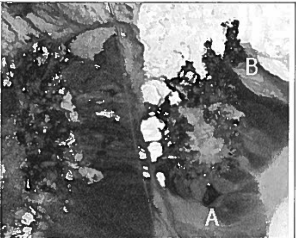
\includegraphics[width=0.5\textwidth]{kaolinite}
\caption{SAM result for Kaolinite in Cuprite, Nevada desert in the USA deribed on an AVIRIS image.}
\label{fig:nevadasam}
\end{figure}

\section{Referenties}
Geef een label aan \emph{de driehoeksongelijkheid}, \emph{de tabel met mineraalcomposities} en \emph{de foto van kaoliniet}. Maak een referentie naar elke. \emph{hint:} gebruik \ltxi{\usepackage[bookmarksnumbered]{hyperref}} en \ltxi{\autoref}.
\begin{itemize}
\item driehoeksongelijkheid: \autoref{eq:driehoek}
\item mineralen tabel: \autoref{table:mineral}
\item kaoliniet: \autoref{fig:nevadasam}
\end{itemize}

\section{Literatuurlijst}
Zoek onderstaande bron op \href{https://scholar.google.com/}{scholar.google.com}, klik op {\LARGE ''}Cite en dan BibTeX. 

Maak nu op Overleaf een nieuw bestand aan met naam \ltxi{literatuur.bib}. Kopieer de BibTeX tekst van Google Scholar naar dit nieuwe bestand.

Citeer deze bron zoals hieronder, en voeg een literatuurlijst toe 

\emph{hint:}
\begin{ltx}
\bibliographystyle{plain}
\bibliography{literatuur.bib}
\end{ltx}

\begin{mdframed}
The hydraulic head distribution in the Polder satisfies the general solution of the well-known \emph{Polder Problem}\cite{alfonso2010}.
\end{mdframed}

\bibliographystyle{plain}
\bibliography{literatuur.bib}

\section{Eindopdracht}
Gebruik het geleerde om het document op de volgende drie pagina's na te maken.

{\Large Hints:}
\begin{enumerate}
\item De marges zijn 2.54cm, het document staat op A4 papier.
\item Maak een \ltxi{\newcommand} aan voor \Ums{} en \Um.
\item Gebruik \ltxi{\usepackage[version=4]{mhchem}} voor chemische formules. Op \href{https://ctan.org/pkg/mhchem}{ctan.org/pkg/mhchem} staat de documentatie (bestand Package documentation).
\item Gebruik de package \ltxi{parskip} zodat er bij aanvang van een nieuwe parafraaf niet wordt ingesprongen
\item Gebruik \ltxi{newpage} direct ná \ltxi{tableofcontents}
\end{enumerate}

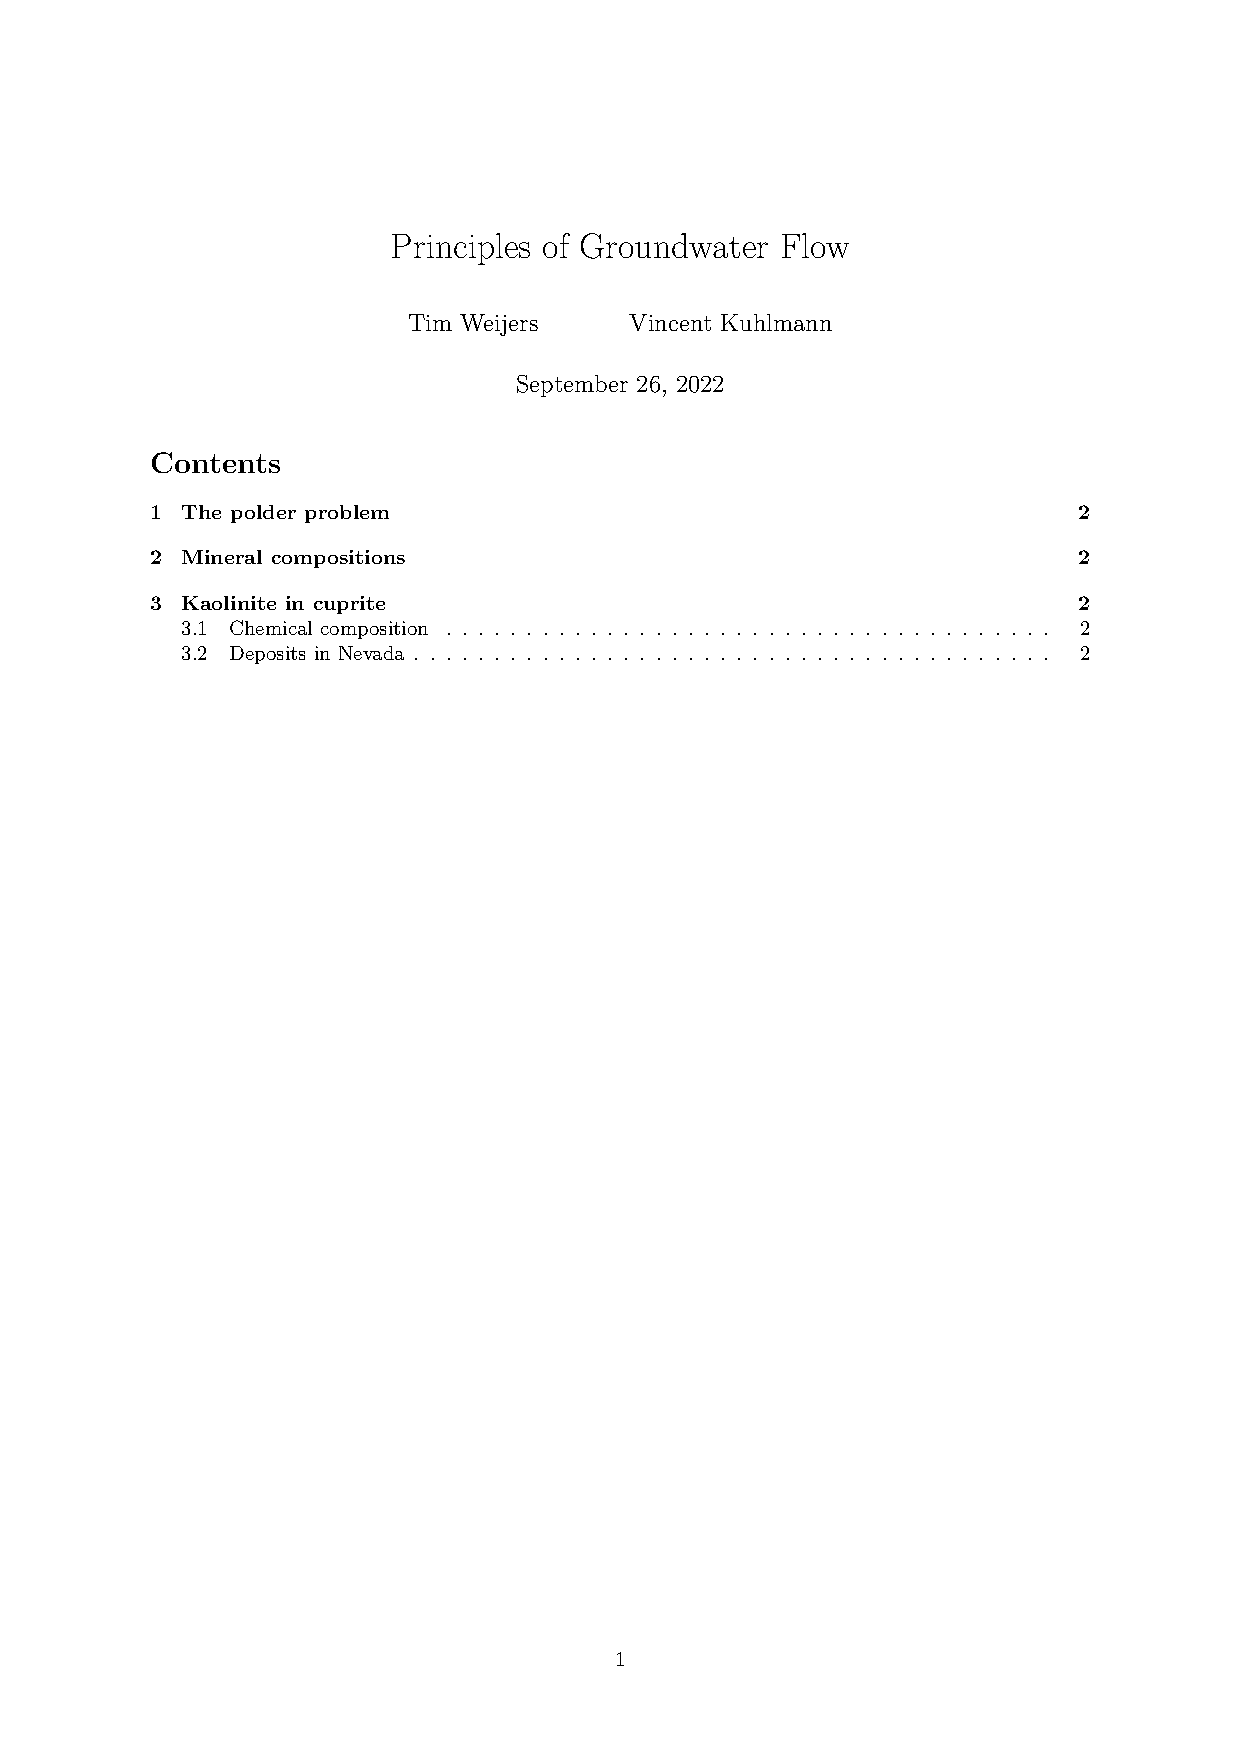
\includepdf[pages=-]{eindopdracht.pdf}





\end{document}